\documentclass[12pt]{article}
\usepackage[dvips]{graphicx}
\topmargin -40pt
\headsep 30pt
\evensidemargin 0pt
\oddsidemargin 0pt
\textwidth 490pt
\textheight 650pt


\def\beq{\begin{equation}}
\def\eeq{\end{equation}}

\begin{document}

%\newpage
\section*{Verdict Triangle Metrics:}

\subsection*{Variable Definitions:}

\begin{figure}[htb]
  \begin{center}
    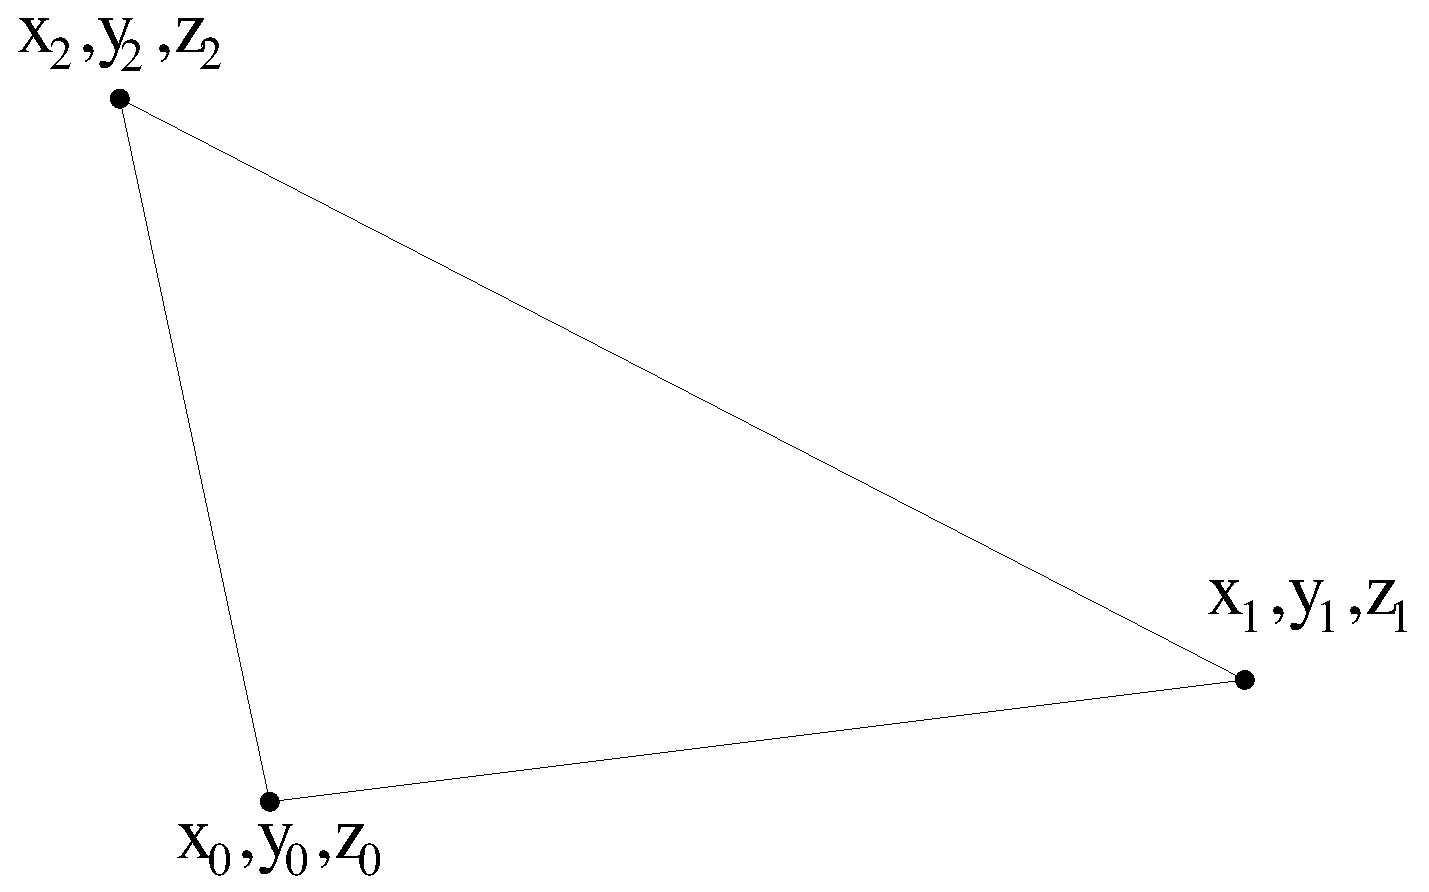
\includegraphics[height=2.0in]{tri.eps}
    \caption{Vertices of Triangle}
    \label{fig:blank}
  \end{center}
\end{figure}

\begin{center}
$\vec P_0 = (x_0, y_0, z_0) $
\end{center}

\begin{displaymath}
\vec P_1 = (x_1, y_1, z_1) 
\end{displaymath}

\begin{displaymath}
\vec P_2 = (x_2, y_2, z_2) 
\end{displaymath}


\begin{displaymath}
A = \frac {| ( \vec P_1 - \vec P_0 ) \times ( \vec P_2 - \vec P_0 ) |}  
          {2} 
\end{displaymath}

\begin{center}
$DBL\_MAX = 1.0E+30 $
\end{center}

\begin{flushleft}
The indices \emph n, (\emph n = 0,1,2), are taken modulo three so that, for example, 
if \emph n = 1, then \emph n + 1 becomes 2 and \emph n + 2 becomes 0.
\end{flushleft}

\subsection*{Overflow:}

\begin{flushleft}
NOTE:  The metrics below are all checked for overflow like so:
\end{flushleft}

\begin{flushleft}
${IF \quad metric\_value > 0;  \quad metric\_value = MIN( metric\_value, DBL\_MAX )}$
\end{flushleft}
 
\begin{flushleft}
${ELSE \quad metric\_value = MAX( metric\_value, -DBL\_MAX )}$
\end{flushleft}

\subsection*{Metric Ranges:}

\begin{flushleft}
Acceptable Range: Well-behaved elements will have metrics in this range.
\end{flushleft}
\begin{flushleft}
Normal Range:     All elements except those with degeneracies will have  \newline
                  metrics in this range.
\end{flushleft}
\begin{flushleft}
Full Range:       All elements including degenerate ones will have metrics \newline
                  in this range. 
\end{flushleft}

%---------------------------Area-----------------------------
\subsection*{Area:}

\begin{displaymath}
\textrm{area} = A 
\end{displaymath}

\begin{tabular}{lll}
& Metric Description:  & (1/2) * Cross-product at any corner node. \\
& Dimension:           & 2                              \\ 
& Acceptable Range:    & 0 to $DBL\_MAX$                      \\ 
& Normal Range:        & 0 to $DBL\_MAX$                      \\ 
& Full Range:          & 0 to $DBL\_MAX$                       \\ 
& Note:                & Since $A$ is non-negative, the currrent version of \\
&                      & Verdict cannot detect inverted triangles. \\
& Reference:           & \cite{three}                     \\ 
\end{tabular} 


%---------------------------Aspect Ratio-----------------------------
\subsection*{Aspect Ratio:}

\begin{displaymath}
aspect~ratio = \frac {{|\vec{P_1} - \vec{P_0} |}^{2} +
                            {|\vec{P_2} - \vec{P_1} |}^{2} + 
                            {|\vec{P_0} - \vec{P_2} |}^{2} }
                            {4A \sqrt{3}}
\end{displaymath}

\begin{tabular}{lll}
& Metric Description:  & Ratio of sum of edge lengths squared to \\
&                      & triangle area. Measures element shape. \\
& Dimension:           & 0                      \\ 
& Acceptable Range:    & 1 to 1.3               \\ 
& Normal Range:        & 1 to $DBL\_MAX$                      \\ 
& Full Range:          & 1 to $DBL\_MAX$ \\ 
& Value of metric on Unit Equilateral Triangle:       & Aspect Ratio = 1.0 \\
& Value of metric on 'Flat' Triangle:  & Aspect Ratio = $DBL\_MAX$ \\
& Note:                & When $A = 0$, Verdict returns \\
&                      & Aspect Ratio = $DBL\_MAX$  \\
& Reference:           &  \cite{one}  \cite{two}  \\
\end{tabular} 

%---------------------------Condition Number-----------------------------
\subsection*{Condition Number:}

\begin{displaymath}
\vec v_1 = {\vec P_1 - \vec P_0}
\end{displaymath}

\begin{displaymath}
\vec v_2 = {\vec P_2 - \vec P_0}
\end{displaymath}

\begin{displaymath}
condition~number = \frac {\Big( (\vec v_1 \bullet \vec v_1) + 
                        (\vec v_2 \bullet \vec v_2) -  
                        (\vec v_1 \bullet \vec v_2) \Big)} 
                        { 2A \sqrt 3 }
\end{displaymath}

\begin{tabular}{lll}
& Metric Description:  & Condition number of weighted Jacobian matrix.         \\
&                      & Measures element shape.   \\
& Dimension:           & 0                      \\ 
& Acceptable Range:    & 1 to 1.3               \\ 
& Normal Range:        & 1 to $DBL\_MAX$        \\ 
& Full Range:          & 1 to $DBL\_MAX$        \\ 
& Value of metric on Unit Equilateral Triangle:       & Condition Number = 1.0 \\
& Value of metric on 'Flat' Triangle:  & Condition Number = $DBL\_MAX$  \\
& Note:                & When $A = 0$, Verdict returns  \\
&                      & Condition Number = $DBL\_MAX$  \\
&                      & Condition Number is invariant to which \\
&                      & node it is computed at. \\
& Reference:           & \cite{four}, \cite{five} \\
\end{tabular} 

%---------------------------Distortion-----------------------------
\subsection*{Distortion:}

\begin{displaymath}
distortion = \frac{ |J|*master\textrm{-}area } { true\textrm{-}area }  
\end{displaymath}

\begin{flushleft} Where, \end{flushleft}
$|J| = $ minimum determinant of the Jacobian computed over all gauss points  \newline
of the element.  The location of the Gauss points is not documented. \newline 
$master\textrm{-}area =$ area of the master tri, where the master tri's corner nodes \newline
are as follows: \newline

 $\vec P_0 = ( -1, -\frac {\sqrt{3}}{3}, 0 )$, 
 $\vec P_1 = ( 1, -\frac{\sqrt{3}}{3}, 0 )$,
 $\vec P_1 = ( 0, \frac{2\sqrt{3}}{3}, 0 )$ \newline

\begin{tabular}{lll}
& Metric Description:  & Minimum Gauss Point Jacobian divided by tri \\
&                      & area, times master tri's area. \\ 
& Dimension:           & $L^0$              \\ 
& Acceptable Range:    & 0.5 to 1            \\ 
& Normal Range:        & 0 to 1        \\ 
& Full Range:          & $-DBL\_MAX$ to $DBL\_MAX$        \\ 
& Value of metric on Unit Equilateral Triangle:       & Distortion = 1.0 \\
& Note:                & This metric is currently unsupported. \\ 
& Reference:           &  Adapted from \cite{six} \\
\end{tabular} 

%---------------------------Maximum Angle-----------------------------
\subsection*{Maximum Angle:}

\begin{displaymath}
\theta_{max}= \arccos{\Bigg( \frac {(\vec P_{n+1} - \vec P_n) \bullet (\vec P_{n-1} - \vec P_n)}
                 {|\vec P_{n+1} - \vec P_n | |\vec P_{n-1} - \vec P_n| } \Bigg) }
                 \Bigg( \frac {180} {\pi} \Bigg)
\end{displaymath}

\begin{flushleft}
where $n$ in $\theta_n$ is the index of the node opposite the longest edge length
\end{flushleft}

\begin{tabular}{lll}
& Metric Description:  & Maximum included angle in triangle. \\
& Dimension:           & degrees                             \\ 
& Acceptable Range:    & 60 to 90                            \\ 
& Normal Range:        & 60 to 180                           \\ 
& Full Range:          & 0 to 180                           \\ 
& Value of metric on Unit Equilateral Triangle:       & $\theta_{max}= 60 $ \\
& Value of metric on 'Flat' Triangle:  & $\theta_{max} = 0 $\\
& Note:                & If $P_0$ = $P_1$ or $P_0$ = $P_2$ or $P_1$ = $P_2$, \\
&                      & Verdict returns $\theta_{max}$ = 0.0  \\
& Reference:           & \cite{three} \\ 
\end{tabular} 


%---------------------------Minimum Angle-----------------------------
\subsection*{Minimum Angle:}

\begin{displaymath}
\theta_{min}= \arccos{\Bigg( \frac {(\vec P_{n+1} - \vec P_n) \bullet (\vec P_{n-1} - \vec P_n)}
                 {|\vec P_{n+1} - \vec P_n | |\vec P_{n-1} - \vec P_n| } \Bigg) }
                 \Bigg( \frac {180} {\pi} \Bigg)
\end{displaymath}

\begin{flushleft}
where $n$ in $\theta_n$ is the index of the node opposite the shortest edge length
\end{flushleft}

\begin{tabular}{lll}
& Metric Description:  & Minimum included angle in triangle. \\
& Dimension:           & degrees                             \\ 
& Acceptable Range:    & 30 to 60                            \\ 
& Normal Range:        & 0 to 60                           \\ 
& Full Range:          & 0 to 360                           \\ 
& Value of metric on Unit Equilateral Triangle:       & $\theta_{min}= 60 $ \\
& Note:                & If $P_0$ = $P_1$ or $P_0$ = $P_2$ or $P_1$ = $P_2$, \\
&                      & Verdict returns $\theta_{min}$ = 360.0  \\
& Value of metric on 'Flat' Triangle:  & $\theta_{min} = 360$ \\
& Reference:           & \cite{three}  \\
\end{tabular} 

%---------------------------Scaled Jacobian-----------------------------
\subsection*{Minimum Scaled Jacobian:}

\begin{displaymath}
L_{max} = MAX( | \vec P_1 - \vec P_0 | * | \vec P_2 - \vec P_1 |, 
               | \vec P_1 - \vec P_0 | * | \vec P_0 - \vec P_2 |, 
               | \vec P_2 - \vec P_1 | * | \vec P_0 - \vec P_2 | )
\end{displaymath}

\begin{displaymath}
IF( \vec surf\_normal_{at~tri~center} \times ( \vec P_0 - \vec P_2 \times \vec P_1 - \vec P_0 ) > 0 )
~~jacobian = -1 * jacobian
\end{displaymath}

\begin{displaymath}
scaled~jacobian = \frac {2 * jacobian } { \sqrt 3 * L_{max} } 
\end{displaymath}

\begin{tabular}{lll}
& Metric Description:  & Jacobian divided by the lengths of 2 longest edges times $\frac{2}{\sqrt 3}$. \\
& Dimension:           & 0                                          \\ 
& Full Range:          & -1.155 to +1.155                           \\ 
& Acceptable Range:    & 0.5 to 1.155                               \\ 
& Note:                & If $L_{max} < DBL\_MIN, scaled~jacobian = 0$ \\
& Reference:           & \cite{four} \\
\end{tabular} 


%---------------------------Relative Size-Squared-----------------------------
\subsection*{Relative Size-Squared:}

\begin{displaymath}
R = \Bigg(\frac {A} {Average \quad Triangle \quad Area} \Bigg)^2
\end{displaymath}
\begin{displaymath}
relative~size \textrm{-}squared = MIN( R, \frac{1}{R} ) 
\end{displaymath}

\begin{tabular}{lll}
& Metric Description:  & Measures ratio of triangle area to average area \\ 
&                      & of all triangles in mesh.             \\ 
& Dimension:           & 0                                          \\ 
& Acceptable Range:    & 0.25 to 1                                     \\ 
& Normal Range:        & 0 to 1                           \\ 
& Full Range:          & 0 to 1                           \\ 
& Value of metric on Unit Equilateral Triangle:   & Any triangle whose area is the same as the \\
&                      & average area over the mesh, \\
&                      & Relative Size-Squared = 1.0  \\
& Value of metric on 'Flat' Triangle:  & Relative Size-Squared = 0.0               \\ 
& Note:                & If $Average$ $Triangle$ $Area$ = 0 or $A$ = 0, \\ 
&                      & Verdict returns Relative Size-Squared = 0.0 \\
& Reference:           & \cite{five} \\ 
\end{tabular} 

%---------------------------Shape-----------------------------
\subsection*{Shape:}

\begin{displaymath}
shape = \frac { 1 } { condition~number }
\end{displaymath}

\begin{tabular}{lll}
& Metric Description:  & 1/Condition Number of weighted Jacobian \\
&                      & matrix. Measures element shape.   \\
& Dimension:           & 0                                          \\ 
& Acceptable Range:    & 0.25 to 1                                     \\ 
& Normal Range:        & 0 to 1                           \\ 
& Full Range:          & 0 to 1                           \\ 
& Value of metric on Unit Equilateral Triangle:       & Shape = 1.0 \\
& Value of metric on 'Flat' Triangle:  & Shape = 0.0  \\
& Reference:           & \cite{five} \\ 
\end{tabular} 

%---------------------------Shape & Size-----------------------------
\subsection*{Shape and Size:}
\begin{displaymath}
  shape~and~size = shape * relative~size \textrm{-}squared 
\end{displaymath}

\begin{tabular}{lll}
& Metric Description:  & Product of Shape and Relative Size \\
& Dimension:           & 0                                  \\ 
& Acceptable Range:    & 0.25 to 1                                     \\ 
& Normal Range:        & 0 to 1                           \\ 
& Full Range:          & 0 to 1                           \\ 
& Value of metric on Unit Equilateral Triangle: & If triangle's area equals the average Area,  \\
&                      & Shape and Size = 1.0 \\
& Value of metric on 'Flat' Triangle:  & Shape and Size = 0.0 \\ 
& Reference:           &  \cite{five} \\
\end{tabular} 



\begin{thebibliography}{99}

\bibitem{one} Bhatia, R.P. and Lawrence, K.L. "Two-dimensional 
finite element mesh generation based on stripwise automatic
triangulation," Computers and Structures, 36:309-319, 1990. 

\bibitem{two} Bank, R.E. and Xu, J.  "An algorithm 
for coarsening unstructured meshes,"Numerische Mathematik, 
73, p1-36, 1996. 

\bibitem{three} Traditional.

\bibitem{four} P. Knupp, "Achieving Finite Element Mesh Quality
via Optimization of the Jacobian Matrix Norm and Quantities", 
Intl. J. Numer. Meth. Engng. 2000, 48:1165-1185.

\bibitem{five} P. Knupp, "Algebraic mesh quality metrics for 
unstructured initial meshes" Finite Elements in Analysis and 
Design, Vol 39, p217-241, 2003. 

\bibitem{six} SDRC/IDEAS Simulation: Finite Element 
Modeling--User's Guide.


\end{thebibliography}

\end{document}
